\let\negmpace\undefined
\let\negthickspace\undefined
\documentclass[journal]{IEEEtran}
\usepackage[a5paper, margin=10mm, onecolumn]{geometry}
\usepackage{tfrupee} % Include tfrupee package
\setlength{\headheight}{1cm} % Set the height of the header box
\setlength{\headsep}{0mm}     % Set the distance between the header box and the top of the text
\usepackage{gvv-book}
\usepackage{gvv}
\usepackage{cite}
\usepackage{amsmath,amssymb,amsfonts,amsthm}
\usepackage{algorithmic}
\usepackage{graphicx}
\usepackage{textcomp}
\usepackage{xcolor}
\usepackage{txfonts}
\usepackage{listings}
\usepackage{enumitem}
\usepackage{mathtools}
\usepackage{gensymb}
\usepackage{comment}
\usepackage[breaklinks=true]{hyperref}
\usepackage{tkz-euclide} 
\usepackage{listings}
\def\inputGnumericTable{}                                 
\usepackage[latin1]{inputenc}                                
\usepackage{color}                                            
\usepackage{array}                                            
\usepackage{longtable}                                       
\usepackage{calc}                                             
\usepackage{multirow}                                         
\usepackage{hhline}                                           
\usepackage{ifthen}                                           
\usepackage{lscape}
\renewcommand{\thefigure}{\theenumi}
\renewcommand{\thetable}{\theenumi}
\setlength{\intextsep}{10pt} % Space between text and floats


\renewcommand{\thetable}{\theenumi}
\begin{document}
\bibliographystyle{IEEEtran}
\title{Question-9-9.2-23}
\author{EE24BTECH11035 - KOTHAPALLI AKHIL}
{\let\newpage\relax\maketitle}
\vspace{-10mm}
\textbf{Question}:\\
Find the area of the region enclosed by the parabola $y^2 = 4x$ and the line $x = 3$.\\
\textbf{Solution}:\\

The general conic form for a parabola $ax^2 + 2bxy + cy^2 + 2dx + 2ey + f = 0$ can be represented by matrices:
\begin{equation}
V = \begin{pmatrix} a & b \\ b & c \end{pmatrix}, \quad u = \begin{pmatrix} d \\ e \end{pmatrix}, \quad f
\end{equation}

For the parabola $y^2 = 4x$,
\begin{equation}
V_{\text{parabola}} = \begin{pmatrix} 0 & 0 \\ 0 & 1 \end{pmatrix}, \quad u_{\text{parabola}} = \begin{pmatrix} -2 \\ 0 \end{pmatrix}, \quad f_{\text{parabola}} = 0
\end{equation}

The line equation can be expressed in matrix form as:
\begin{equation}
h^T x + m = 0
\end{equation}
Where $h$ is the vector of coefficients and $m$ is the constant.

For $x = 3$,
\begin{equation}
h_{\text{line}} = \begin{pmatrix} 1 \\ 0 \end{pmatrix}, \quad m_{\text{line}} = -3
\end{equation}
Substituting $x = 3$ into the parabola equation $y^2 = 4x$:
\begin{equation}
y^2 = 4(3) = 12
\end{equation}
\begin{equation}
y = \pm 2\sqrt{3}
\end{equation}
The points of intersection are $\begin{pmatrix} 3 \\ 2\sqrt{3} \end{pmatrix}$ and $\begin{pmatrix} 3 \\ -2\sqrt{3} \end{pmatrix}$.\\
Calculating area between parabola and line from $y = -2\sqrt{3}$ to $y = 2\sqrt{3}$ is:
\begin{equation}
\text{Area} = 2 \int_{0}^{2\sqrt{3}} \left( 3 - \frac{y^2}{4} \right) \, dy
\end{equation}
\begin{equation}
\int \left( 3 - \frac{y^2}{4} \right) \, dy = 3y - \frac{y^3}{12}
\end{equation}

Substituting the limits,
\begin{equation}
\left[ 3y - \frac{y^3}{12} \right]_{0}^{2\sqrt{3}} = 3(2\sqrt{3}) - \frac{(2\sqrt{3})^3}{12}
\end{equation}
\begin{equation}
= 6\sqrt{3} - \frac{8(3\sqrt{3})}{12} = 6\sqrt{3} - 2\sqrt{3} = 4\sqrt{3}
\end{equation}

Thus, the area of the region enclosed by the parabola and the line is:
\begin{equation}
\text{Area} = 2 \times 4\sqrt{3} = 8\sqrt{3} \, \text{square units}.
\end{equation}
\begin{figure}[h!]
	\centering
	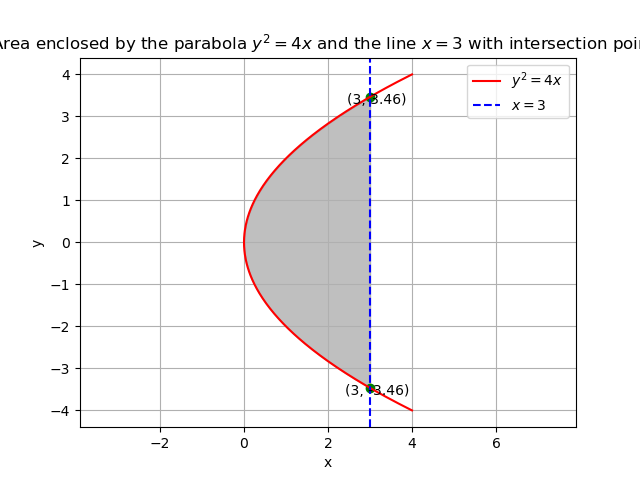
\includegraphics[width=0.5\linewidth]{figs/Figure_1.png}
	\caption{Area enclosed between parabola and Line}
	\label{stemplot}
\end{figure}	

\end{document}

